\chapter{atc}\label{sec:atc}

atc \cite{atc} is a C++ tool for parsing C/C++ code into comparatree, primarily developed as part of a research project preceding this thesis, and later slightly changed to fulfill new interface requirements of comparatree and the whole project.
See the documentation of atc in the research project for more details.

atc would also be used in another diploma thesis, that needs semantic information from the code.
This led to choosing the LibTooling library \cite{libtooling} from clang, which lets us create a standalone tool for parsing C++ code and extracting the relevant information from the ASTs.

The main structure of atc is standard for a clang-based tool.
We define a class \verb|AtcConsumer| that inherits from \verb|ASTConsumer|, which accepts a translation unit and processes it.
The processing is done by a class \verb|AtcVisitor| that inherits from \verb|RecursiveASTVisitor|, which provides a convenient way to traverse the abstract syntax tree (AST) generated by clang and visit each node.
We only need to override the concrete visit methods for the AST nodes that we want to capture in comparatree, collect the interesting information from the AST nodes, and build the corresponding comparatree structures.

\SaveVerb{verb:recursiveastvisitor}|RecursiveASTVisitor|
\begin{figure}[h]
  \centering
  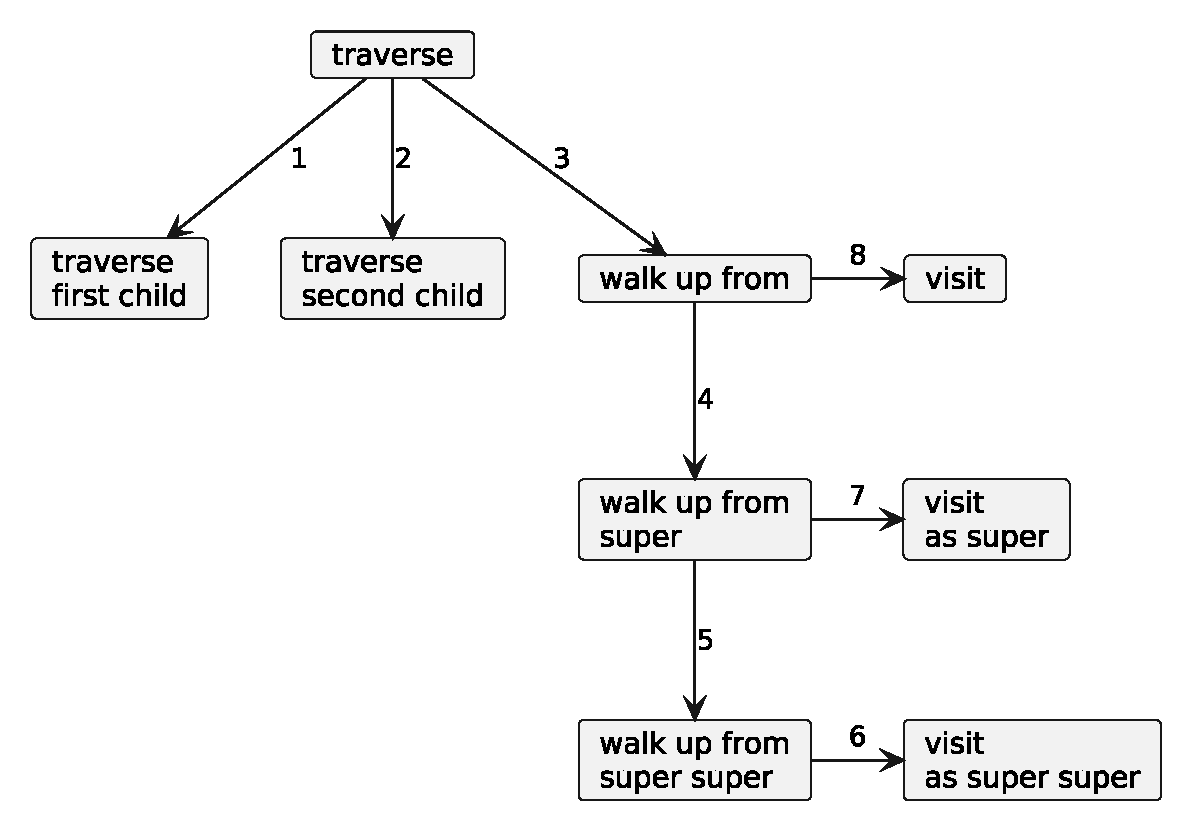
\includegraphics[width=\textwidth]{img/atc-recursive-visitor.eps}
  \caption{Default call graph in \protect\UseVerb{verb:recursiveastvisitor}. The numbers indicate the order of calls.}
  \label{fig:atc-recursive-visitor}
\end{figure}

The \verb|RecursiveASTVisitor| class provides different traversal approaches, see \autoref{fig:atc-recursive-visitor}.
We will refer only to the postorder traversal, which we prefer for comparatree.
\begin{itemize}
\item The \verb|Traverse*| methods are called for each AST node automatically, as they call traversal methods for all the children of the node, and then call the corresponding \verb|WalkUpFrom*| method for the node itself.
\item The \verb|WalkUpFrom*| methods call a \verb|WalkUpFrom*| method for a superclass of the node, and then call the corresponding \verb|Visit*| method for the node itself.
\item The \verb|Visit*| methods are empty.
\end{itemize}

The user can override any of the methods.
We choose to leave the \verb|Traverse*| methods unchanged, as they provide the desired traversal order and behavior.
We override the \verb|WalkUpFrom*| methods to capture the needed information from the AST nodes and we do not include the calls to the superclass methods and the calls to the \verb|Visit*| methods.
This leads to visiting each node only once.
If we did not override some specific \verb|WalkUpFrom*| method, it would call the superclass method and then its superclass method, and so on, until it reaches a \verb|WalkUpFrom*| method that we did override and we can collect at least some information from the node.

We can also use the hierarchy of the node classes for extracting different levels of information about the node.
Each class adds some specific information on top of the information captured by its superclasses.
We capture the node class specific information and call the superclass extracting method to capture the whole information about the node.

We also build the type descriptors according to the type hierarchy of the AST node classes.

\section{Statistics}

Copy from project or create new ones??
